\documentclass{article}

\usepackage{geometry}
\geometry{margin=2cm}
\usepackage{graphicx}
\usepackage{hyperref}
\usepackage{amsfonts}
\usepackage{caption}
\usepackage{subcaption}

\hypersetup{colorlinks=true, linkcolor=blue, urlcolor=blue}
\urlstyle{same}
\begin{document}
	
	\author{Aayush Arya}
	\date{(Submitted: \today)}
	\title{}
	
	\maketitle
	
	\hrule
	\begin{center}
		PHY350 Lab Report\\
		Practical: 8 \quad Registration No.: 11912610 \quad Section: G2903
	\end{center}
	\hrule
	
	\section*{Aim}
	To measure the hall coefficient and carrier concentration of a semiconductor sample.
	
	\section*{Results \& Conclusions}
	
	For the chosen $0.5$mm thickness Ge sample, the hall coefficient was found to be $R_H=0.01939$ and the carrier concentration was $n = 3.221 \times 10^{20}$.
	
	The data has been plotted in the figure below.
	
	\begin{figure}[!h]
		\centering
		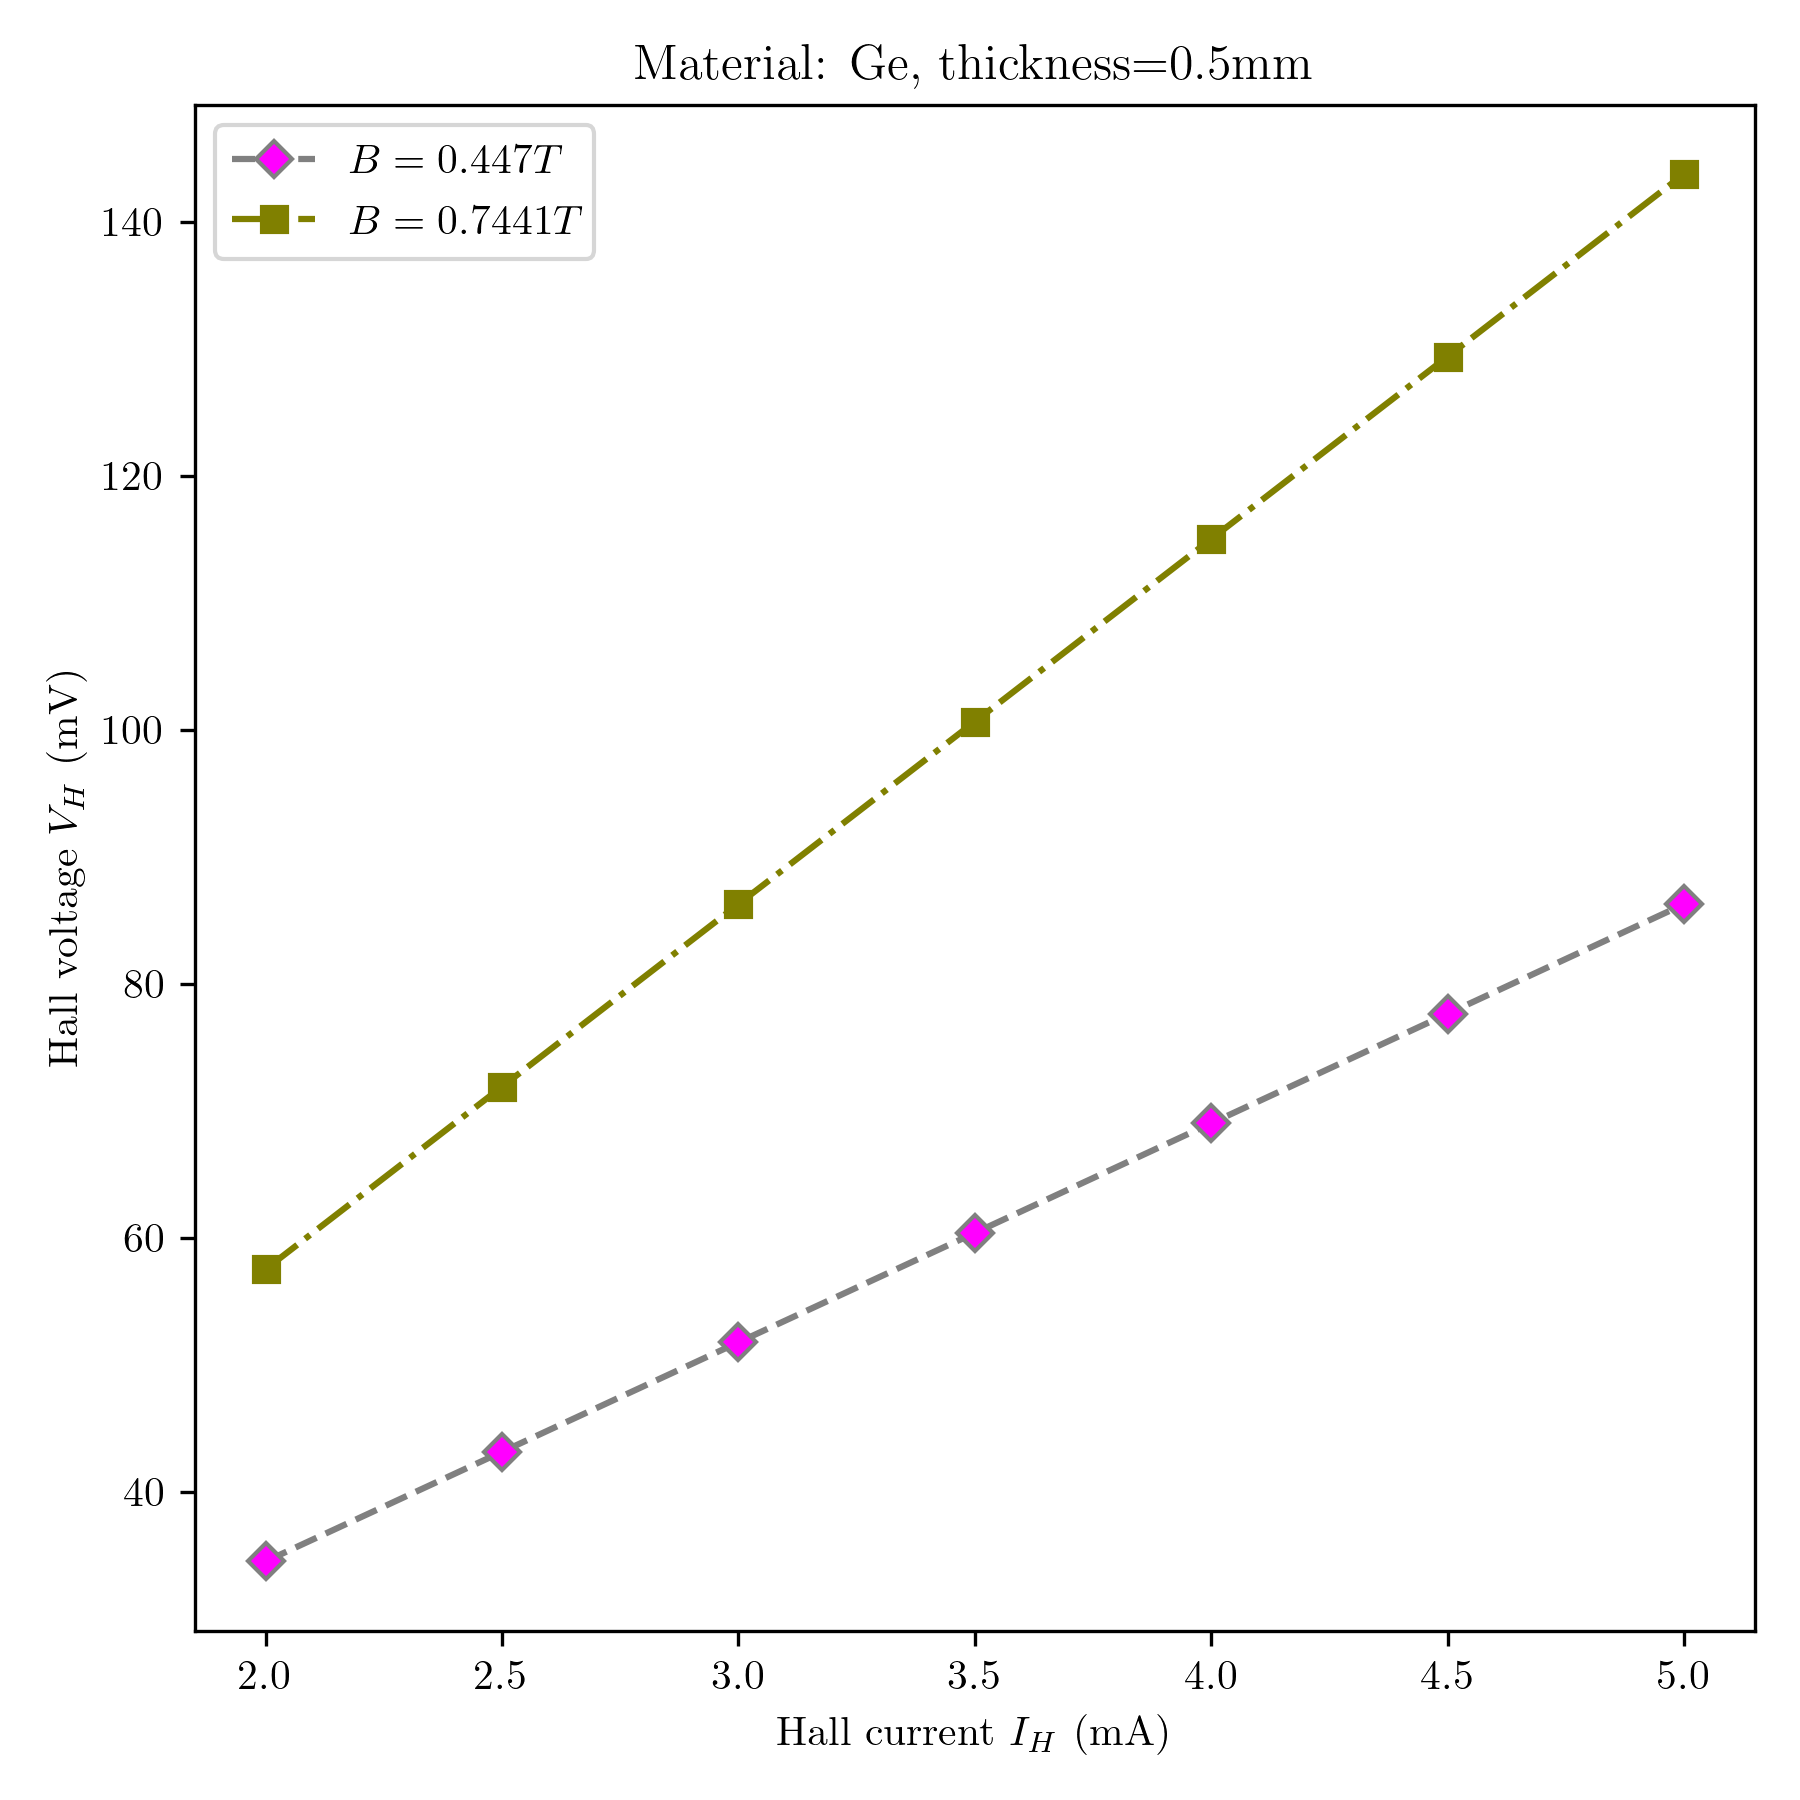
\includegraphics[width=0.6\textwidth]{hall_effect}
		\caption{Plot of hall voltage vs current}
	\end{figure}

	The values measured are as follows

	\begin{table}[h]
		\centering
		\begin{tabular}{|c|c|c|}
			\hline
			Hall current & $V_H$ ($B=0.4447$) & $V_H$ ($B=0.7441 $)\\
			\hline
			2.0 & 34.507 & 57.511\\
			2.5 & 43.133 & 71.889\\
			3.0 & 51.760 & 86.267 \\
			3.5 & 60.387 & 108.645\\
			4.0 & 68.014 & 115.625\\
			4.5 & 77.640 & 129.4 \\
			5.0 & 86.267 & 143.778\\
			\hline
		\end{tabular}
		\caption{Measurements for Ge, thickness=0.5mm}
	\end{table}
	
	
	Since the hall voltage and hall current are related by $$ V_H = \frac{R_H I B}{t} $$ where $$ R_H = \pm \frac{1}{ne}$$
	The values for $R_H$ and $n$ could be estimated from the slope of the data.\\
	
	The calculated values of $R_H$ and carrier concentration $n$ are $0.01939$ and $3.221\times 10^{20}$ respectively.\\
	
	
\end{document}